% Chapter Template

\chapter{Traditional Uncertainty Quantification Methods} % Main chapter title

\label{ch:methods basic} % Change X to a consecutive number; for referencing this chapter elsewhere, use \ref{ChapterX}

\lhead{Chapter 2. \emph{Methods: Traditional UQ}} % Change X to a consecutive number; this is for the header on each page - perhaps a shortened title

%----------------------------------------------------------------------------------------
%	SECTION: INTRO
%----------------------------------------------------------------------------------------

\section{Introduction}
In this chapter we describe traditional uncertainty quantification concepts as well as several common existing
uncertainty quantification methods and their applications.
We begin
by discussing the principles of input spaces and responses, and define terminology used in this work.  Next we
discuss uncertainty quantification at a high level, and finally describe several common uncertainty quantification
tools.

% inputs and outputs
Many simulation models are algorithms constructed to solve partial differential equations, often in two or
three spatial dimensions and possibly time.  The inputs to these models include boundary conditions, material
properties, tuning parameters, and so forth.  The outputs are responses, either data fields or
scalar values.  The responses are used to inform decision-making processes.  For example, a neutronics
simulation in nuclear engineering takes materials, geometries, and boundary conditions as inputs, and yields
neutron flux and the neutron multiplication factor $k$ as responses.  Similarly, a fuels performance code
takes materials, geometries, and power shapes as inputs and yields stresses, strains, and temperature profiles
as outputs.  Figure \ref{fig:ober} is an example of this workflow \cite{oberkampf}.
\begin{figure}
  \centering
  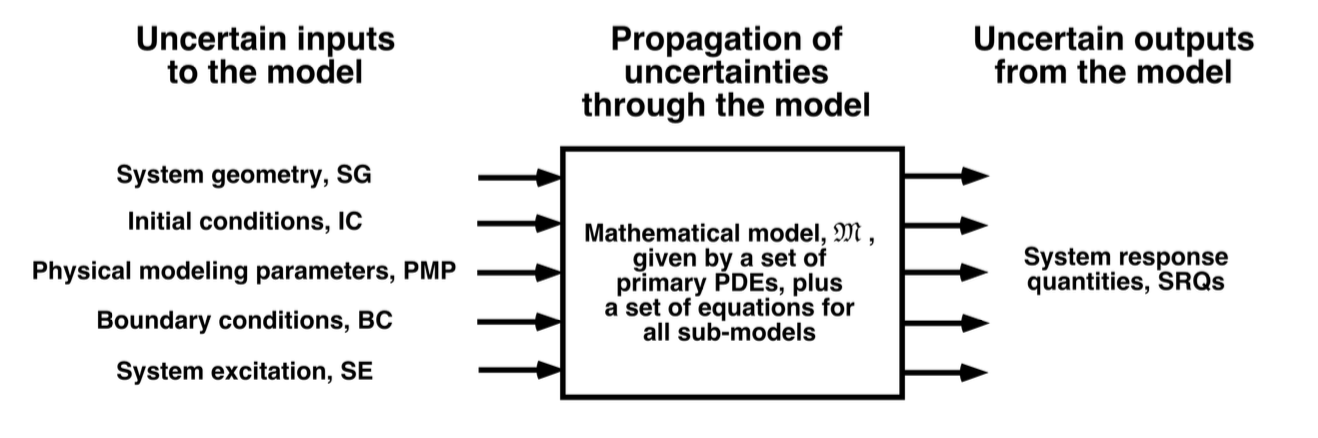
\includegraphics[width=\linewidth]{v_and_v_uq}
  \caption{Uncertainty Quantification \cite{oberkampf}}
  \label{fig:ober}
\end{figure}

In general, we define $u(Y)$ to be
a response as a function of the input space $Y = (y_1,\ldots,y_n,\ldots,y_N)$ where $y_n$ is a single
uncertain input
parameter to the model, $n$ is an index spanning the number of inputs, and $N$ is the total number of inputs.
Uncertain input parameters can include any of the inputs to the simulation.
We assume each response to be a scalar, integrated quantity.  In the event
the output is a vector or field quantity, each element can be considered as a distinct scalar response.
\emph{Models} are mathematical equations used to obtain the response $u(Y)$, and \emph{solvers} or
\emph{simulations} are numerical algorithms used to solve models.

Using our examples above, for neutronics calculations $Y$ might include nuclear cross sections, geometry
parameters, and sources, while $u(Y)$ could be $k$-effective or the neutron flux at a particular location of
interest.  For fuels performance calculations, $Y$ might entail thermal conductivity of various parameters,
geometric construction parameters, moderator inlet temperatures, and so forth.  $u(Y)$ could be peak clad
temperature, maximum fuel centerline temperature, clad elongation, percent fission gas released, and so on.

\subsection{Uncertain Inputs}
Essential to using simulation models is understanding the possibility that significant uncertainties existing in
the inputs.  These could be aleatoric uncertainties due to intrinsic randomness in the inputs, or epistemic
uncertainties due to model imperfections or lack of knowledge.  
For example, quantum behaviors or Brownian motion often provide non-deterministic sources of aleatoric uncertainty.
Further, the simulation itself might be solved through non-deterministic methods such as Monte Carlo sampling,
in which case the random seed acts as an uncertain input.  Examples of epistemic uncertainties include initial
or boundary conditions that can only be controlled to some finite level, such as manufacturing tolerances,
temperature and pressure, and so forth.
Each of these aleatoric and epistemic uncertainties has some
distribution defining the likelihood of an input to have a particular value.  Sometimes these distributions
are known; often, they can only be approximated.  These distributions might be
assumed or constructed from experiment; for our work, we will assume distributions are given, and that the given 
distributions are accurate.  The
input likelihood distribution is the probability distribution function (PDF) $\rho_n(y_n)$.  
An integral over any portion of the input space of the PDF provides the probability that the input's value
is within that portion.
We require
\begin{equation}
  \int_a^b \rho_n(y_n) d\ y_n = 1,
\end{equation}
where $a$ and $b$ are the minimum and maximum values $y_n$ can take (possibly infinite).  In other words, the
probability of finding the input between $a$ and $b$ is 100\%; similarly, we can say the value of the input
lies between $a$ and $b$ almost surely.

\subsection{Multidimensional Input Spaces}
% multidimensional
When there are more than one uncertain input, the combination of distributions for these inputs span an
uncertainty space $\Omega$. $\Omega$ is a part of the probability space $(\Omega,\sigma,\rho)$, where $\Omega$
is the set of all possible outcomes, $\sigma$ is the set of events $\omega$, and $\rho$ is the probability function for
the space.  The dimensionality of $\Omega$ is $N$,
the number of uncertain input variables.  The probability of any event in the input space occurring is given
by an integral of the joint-probability distribution $\rho(Y)$, still enforcing
\begin{equation} \label{eq:joint pdf}
  \int_{a_1}^{b_1}\cdots\int_{a_N}^{b_N} \rho(Y) dy_1\cdots dy_N = 1.
\end{equation}
For clarity, we define multidimensional integral operator
\begin{equation}\label{eq: no rho}
  \int_\Omega (\cdot)dY\equiv \int_{a_1}^{b_1}\cdots\int_{a_N}^{b_N} (\cdot) dy_1\cdots dy_N,
\end{equation}
so that Eq. \ref{eq:joint pdf} can be written
\begin{equation}
  \int_\Omega \rho(Y) dY = 1.
\end{equation}
The function $u(Y)$ maps realizations ($\omega$) from the input space $\Omega$ to a real-valued response.
That is, for each input variable $y_n$, a realization is taken by selecting a single value from the
distribution of $y_n$, which gives a single input value $y_n(\omega)$.  Taking a single realization of each of
the distributed input parameters yields a full input realization $Y(\omega)=(y_1(\omega),\cdots,y_N(\omega))$,
which can be used as inputs for
$u(Y)$ to obtain a realization of the response $u(Y(\omega))$.  To simplify notation, in general the
dependency of a realization on $\omega$ will be omitted and referred to as \emph{sampling} or \emph{taking a
realization}.

% correlation
\subsection{Correlation and the Karhunen-Loevre expansion}\label{sec:KL}
We note the possibility that multiple inputs may be correlated with each other.  When inputs are not
independent, the joint probability distribution is not the product of each individual probability distribution
distribution.  When this is the case, each distribution cannot be sampled independently, and this
creates complications for many of the sampling strategies presented in this work.  

Using input space mapping, however, a surrogate orthogonal input space can be
constructed.  This surrogate space is functionally identical to the original for our purposes.
There are mathematical approaches to decoupling input parameters through surrogate
spaces.  In particular, using principle component analysis (or Karhunen-Loeve expansion
\cite{karhunen} for discrete inputs), the covariance matrix for the distributed input parameters
can be used to construct a multidimensional
standard Gaussian normal distribution, whose components are all orthogonal.
As a result, we only consider independent variables in this work, as dependent variables can
be decoupled through this surrogate mapping process.


\section{Uncertainty Quantification}
% introduction
The purpose of uncertainty quantification is to propagate the uncertainties present in the input space of a
model through that model and comprehend their effects on the output responses.  This is desirable because
single-realization simulations give a very limited view of real-life operation.  In traditional simulations, a
single value for each input variable results in a single value for the response.  When performing uncertainty
quantification, a range of values for each input results in a range of response values.  To quantify the
distribution of the output response, often statistical moments are used, including the mean, variance,
skewness, and kurtosis.

\subsection{Statistical Moments}\label{sec:stat moments}
The four most basic statistical moments used in describing probability distributions are the mean, variance,
skewness, and (excess) kurtosis.
The mean ($\mu$) provides the expected value of the response, or generally the most probable
value for the response.  The variance ($\sigma^2$) establishes the spread of the response, or the distance response values
have from the mean on average.  The standard deviation of the response is given by the square root of the
variance, and provides a useful metric to determine the probability of finding a response value within a
range.  For instance, Chebyshev's inequality \cite{chebyshevineq} says $1-1/k^2$ of a distribution's values
are within $k$ standard deviations from the mean.  This is true whenever the mean and variance can be
defined.  Table
\ref{tab:cheby stdev} shows the minimum percent of the response covered by including multiples of the
standard deviation from the mean.
Some distributions are much more restrictive than Chebyshev's inequality requires.  For instance, we 
show a similar table for a normal Gaussin distribution in Table \ref{tab:norm stdev}.  Fig. \ref{fig:stdev pct}
shows the same information graphically.
\begin{table}[htb]
  \centering
  \begin{tabular}{c c}
  Number of Std. Dev. & Percent of Values \\ \hline
  1 & 0 \\
  $\sqrt{2}$ & 50 \\
  2 & 75 \\
  3 & 88.89 \\
  4 & 93.75 \\
  5 & 96 \\
  10 & 99
  \end{tabular}
  \caption{Percentage of Values within $k$ standard deviations for general distributions}
  \label{tab:cheby stdev}
\end{table}
\begin{table}[htb]
  \centering
  \begin{tabular}{c c}
  Number of Std. Dev. & Percent of Values \\ \hline
  1 & 68.3 \\
  2 & 95.45 \\
  3 & 99.73 \\
  4 & 99.994 \\
  \end{tabular}
  \caption{Percentage of Values within $k$ standard deviations for Gaussian normal}
  \label{tab:norm stdev}
\end{table}
\begin{figure}[H]
  \centering
  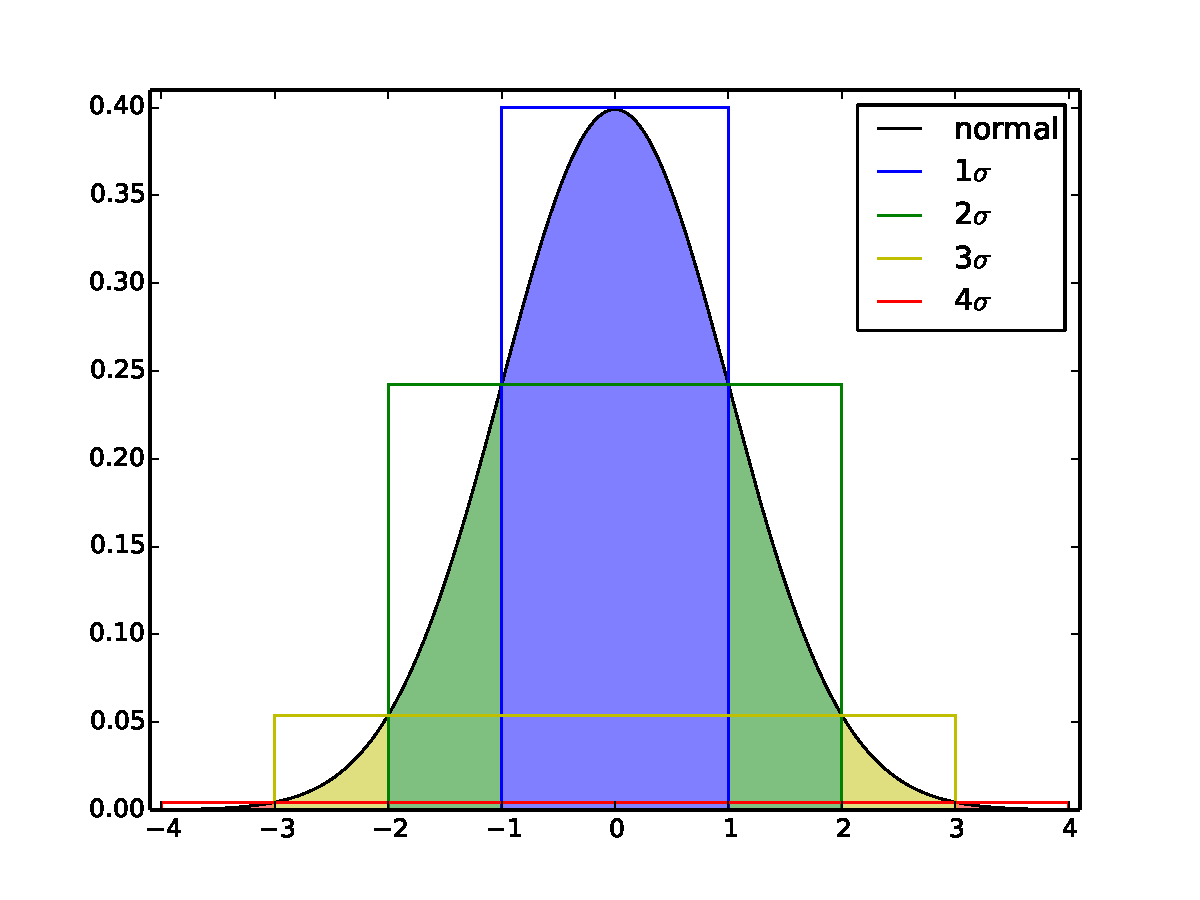
\includegraphics[width=0.7\linewidth]{stdev_pct}
  \caption{Standard Deviations of Normal Gaussian Distribution}
  \label{fig:stdev pct}
\end{figure}
Higher order moments, skewness ($\gamma_1$) and kurtosis ($\gamma_2$), describe the asymmetry and "tailedness"
of the response distribution respectively.  The more asymmetric the distribution, the
higher the skewness is.  For example, a Gaussian normal distribution has zero skewness,
and skewness is introduced to a Beta distribution by allowing $\alpha\neq\beta$.
Kurtosis is more complicated in its interpretation, but in general kurtosis provides an idea
of how much of the variance is contributed by extreme deviations from the mean.  The kurtosis
of a Guassian normal distribution is 3.  This leads to the definition of excess kurtosis,
which is 3 less than the traditional kurtosis.  

An example of similar distributions with different moments is
given in Figure \ref{fig:change moments}.  The mean shifts the entire distribution, the variance spreads the
distribution, the skewness measures asymmetry, and the kurtosis measures tailedness.  In each case, the blue
is a ``standard'' distribution, and the red demonstrates increasing the indicated statistical moment.
\begin{figure}[H]
  \centering
  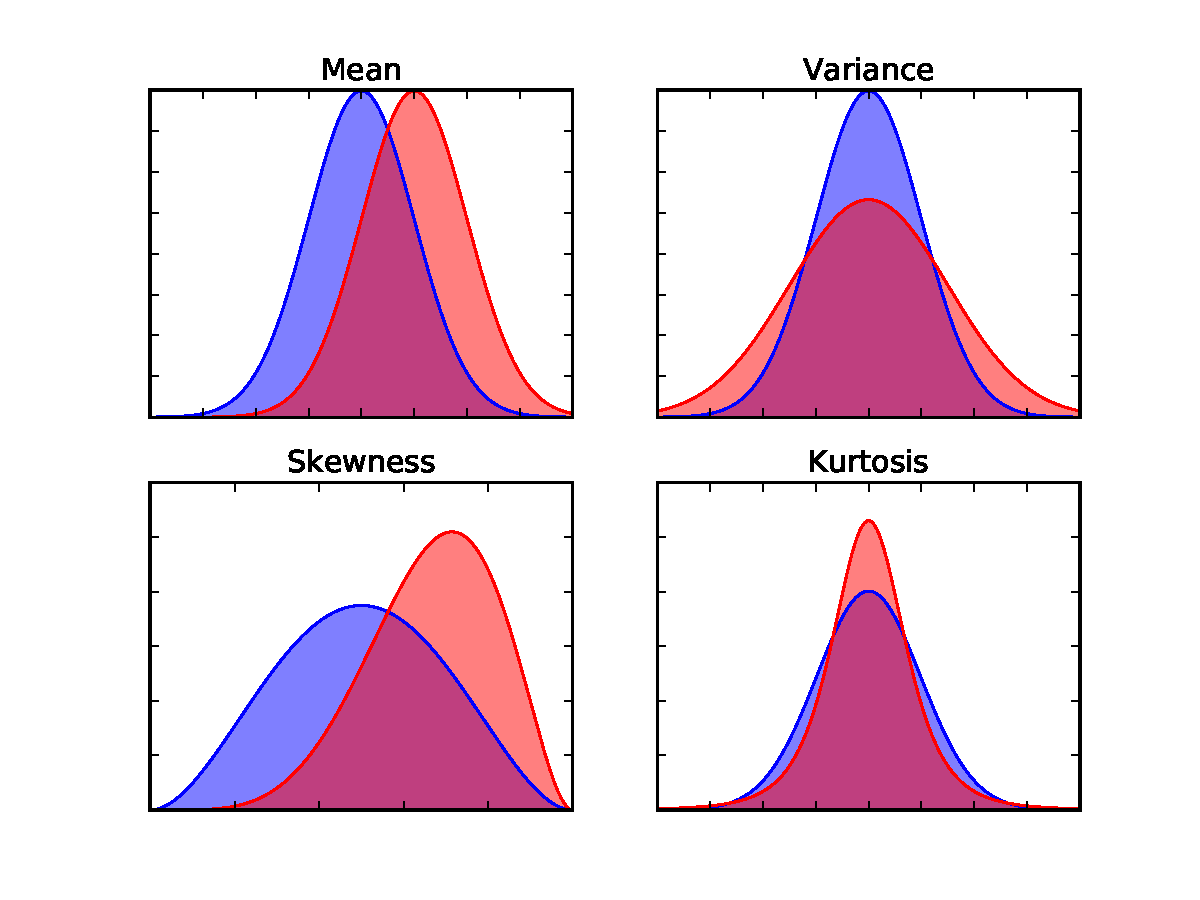
\includegraphics[width=0.7\linewidth]{change_stats}
  \caption{Visual Representation of Statistical Moments}
  \label{fig:change moments}
\end{figure}

While both skewness and kurtosis provide insight to the distribution of responses,
most uncertainty quantification is centered on second-order metrics.
Second-order uncertainty quantification seeks for the mean and variance of
the perturbed response.  Mathematically, the mean of a model is the first moment,
\begin{equation}
  \text{mean} = \expv{u(Y)} = \int_\Omega \rho(Y) u(Y) dY,
\end{equation}
and the variance is the second moment less the square of the first,
\begin{equation}
  \text{variance} = \expv{u(Y)^2} - \expv{u(Y)}^2 = \int_\Omega \rho(Y) u(Y)^2 dY - \text{mean}^2.
\end{equation}
 
Another use for uncertainty quantification is understanding the sensitivity of the output responses to the
uncertain inputs; that is, determining how responses change as a function of changes in the input space.  At
the most primitive level, linear sensitivity of the mean of a response to an input is the derivative of the response
with respect to the input.  Sensitivities can be either local to a region in the input space or global
to the entire space.

There are two chief methods to define sensitivity.  One of the most typical sensitivities
is mean to mean; that is, the rate of change in the value of the response as a function of changes in the
input values.  This metric is most useful what attempting to maximize or minimize a response value by changing
input parameters.  The second method is variance to variance, or the rate of change in the variance of the
response as a function of changes in the variance of an input.  This is useful when trying to mitigate the
spread of possible response values.  If there is a possibility of a response having an undesirable value,
knowing the variance-variance sensitivity helps in identifying which inputs need to have their variance
reduced to prevent the undesirable value from occurring.

\subsection{After Uncertainty Quantification}
Once the response distribution is well-understood through statistical moments and sensitivities, 
further analysis
and decisions can be made.  For example, one post-uncertainty quantification analysis is \emph{limit
surface} definition and \emph{failure probability}.  In this type of analysis, a criteria is given that determines
a ``success'' and ``failure'' condition for a response.  For instance, in the simulation of a
material undergoing stress during heating, a failure condition could be whether the material
buckles during the simulation.  The limit surface search seeks to determine what portion of the
input space results in response failures, and what portion to successes, and define the hypersurfaces dividing
successes and failures.  Figure \ref{fig:lss} shows a sample limit surface search sampling, and Figure
\ref{fig:lss fail} shows the surface between success and failure regions \cite{raven}.  

\begin{figure}[htb]
  \centering
  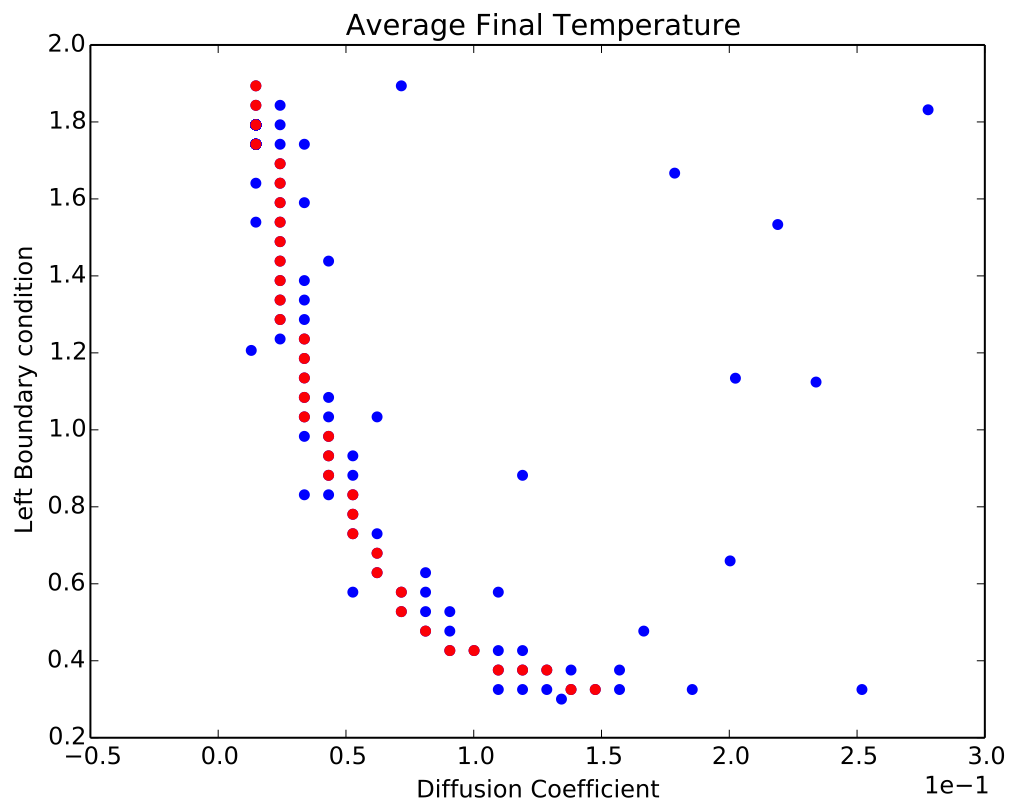
\includegraphics[width=0.5\linewidth]{lss}
  \caption{Limit Surface Sampling \cite{raven}}
  \label{fig:lss}
\end{figure}
\begin{figure}[htb]
  \centering
  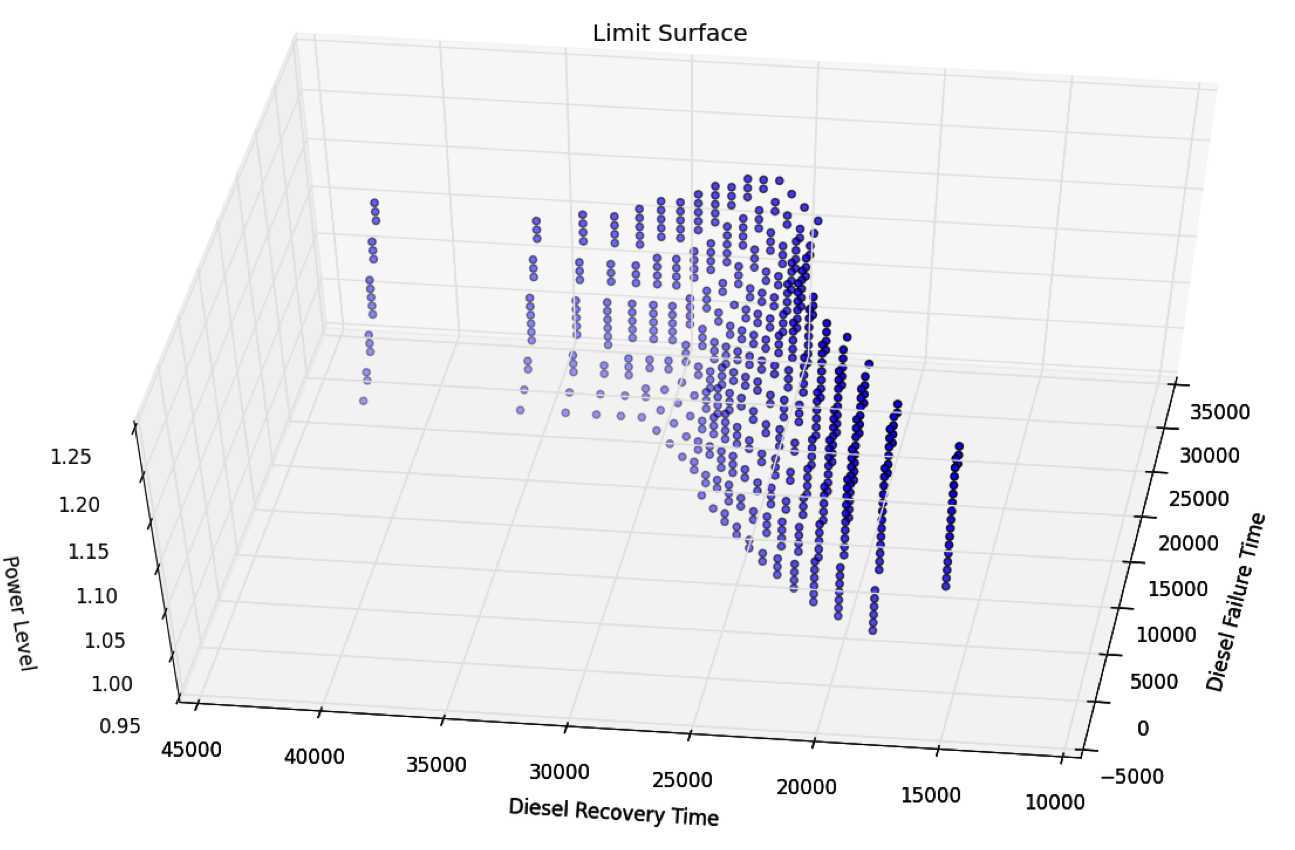
\includegraphics[width=0.7\linewidth]{lss_fail}
  \caption{Limit Surface and Failure Regions \cite{raven}}
  \label{fig:lss fail}
\end{figure}

After a limit surface search, optimization can be performed, which gives
some criteria for ideal operation and searches the success space for optimal inputs.  For example,
if alloy compositions are the inputs for the stress and heat material mentioned earlier, optimization
can help find the least expensive alloy that won't buckle in the conditions given by the simulation.

Another post-uncertainty quantification calculation is to make use of sensitivity information to determine
the inputs that could benefit from reduced variance to reduce the variance of the response in turn.
If some inputs have minimal impact on variance in the output, they don't need the same level of care
in manufacturing as other inputs.  For example, consider the construction of a commercial nuclear power
reactor.  If the material properties and geometry of the reflector have a much smaller impact on the operation
variance than the fuel content and geometry of the fuel pellets, the most naive cost-effective way to control
variance is to decrease margins in fuel manufacturing instead of reflector construction.  While this example
seems readily evident, often engineering intuition can be informed by uncertainty quantification and
sensitivity analysis.

\subsection{Analytic Uncertainty Quantification}
For some models, there exists analytic techniques for propagation of uncertainty.  One of these is the
so-called \emph{sandwich formula}, often referred to as \emph{standard propagation of error} \cite{sandwich}.
Assuming independent input parameters (see section \ref{sec:KL}), the standard deviation $\sigma_u$ of $u(Y)$
is given as
\begin{equation}
  \sigma^2_u = \sum_{n=1}^N \qty(\pdv{u(Y)}{y_n})^2\sigma_{y_n}^2,
\end{equation}
where $\sigma_{y_n}$ is the standard deviation of uncertain input $y_n$.  This approximation is limited to the
linear characteristics of the gradient of $u(Y)$, and so is useful especially when the standard deviation of
the inputs are small compared to the partial derivatives \cite{sandwich2}.

For models with gradients that are simple to calculate accurately (and sufficiently small input
uncertainties), this formula is very effective at propagating error.  However, computing or estimating such
gradients accurately for complex models is prohibitive, and leads to numerical approaches to uncertainty
quantification, as we discuss in this thesis.


\subsection{Uncertainty Quantification Techniques}
There are several common tools used for uncertainty quantification when analytic analysis is not possible or
not practical.
These include stochastic methods such as Monte Carlo sampling, deterministic methods such as Grid sampling,
and mixed methods such as Latin Hypercube sampling (LHS). We discuss each here and show examples of the
sampling strategies.

\subsection{Monte Carlo}
The Monte Carlo method (MC) \cite{mc} has been used formally since the 1930s as a tool to explore possible outcomes
in uncertain models.  Nuclear physicist Enrico Fermi used the method in his work with neutron moderation in
Rome \cite{mcfermi}.  In its simplest form, MC involves randomly picking realizations from a set of
possibilities, then statistically collecting the results.  In uncertainty quantification, Monte Carlo can be
used to sample realizations in the input space based on the joint probability distribution.  These
realizations are then run through the model solver, and the collection of
response realizations is analyzed to determine its moments.

The mean of a response is determined by MC using the unweighted average of samples collected:
\begin{equation}
  \expv{u(Y)} = \frac{1}{M}\sum_{m=1}^M \qty(u(Y(\omega_m))) + \epsilon_M^{\text{MC}},
\end{equation}
where $Y(\omega_m)$ is a realization randomly chosen based on $\rho(Y)$, and $M$ is the total number of samples taken.
The error in the approximation diminishes with the root of the number of samples taken,
\begin{equation}
  \epsilon_M^{\text{MC}} \propto \frac{1}{\sqrt{M}}.
\end{equation}
The second moment is similarly approximated as
\begin{equation}
  \expv{u(Y)^2} \approx \frac{1}{M}\sum_{m=1}^M \qty(u(Y(\omega_m))^2).
\end{equation}
The standard deviation (root of the variance) converges similarly to the mean for Monte Carlo methods.  There
are many tools that can be used to improve Monte Carlo sampling \cite{mcvarred}\cite{mcnpvarred}; we restrict
our discussion to traditional analog Monte Carlo sampling.

Monte Carlo has long been a gold standard for uncertainty quantification because of its consistency.  Monte
Carlo will always resolve the response statistics given a sufficient number of samples.  Additionally, the
convergence of Monte Carlo is largely agnostic of the input space dimensionality, a feature not shared by the
Grid sampling method.

The drawback to Monte Carlo sampling also centers on its consistency.  The error in analog Monte Carlo can only be
consistently reduced by drastically increasing the number of evaluations solved.  While coarse estimates are
inexpensive to obtain, high precision takes a great deal of effort to converge.
Figure \ref{fig:mc sample}
shows Monte Carlo sampling of a two-dimensional input space, and Figure \ref{fig:mc prob} shows the
probability weight of the sampled points \cite{raven}.

\begin{figure}[H]
  \centering
  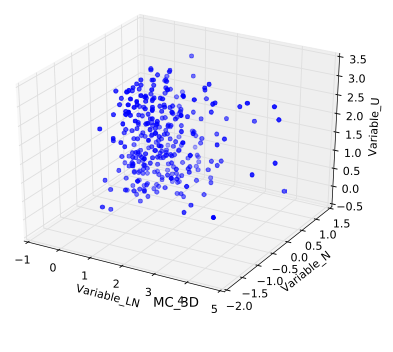
\includegraphics[width=0.5\linewidth]{mc_sample}
  \caption{Example Monte Carlo Samples \cite{raven}}
  \label{fig:mc sample}
\end{figure}
\begin{figure}[H]
  \centering
  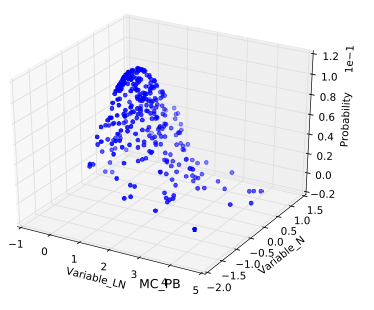
\includegraphics[width=0.5\linewidth]{mc_prob}
  \caption{Example Monte Carlo Probabilities \cite{raven}}
  \label{fig:mc prob}
\end{figure}

\subsection{Grid}
One of the drawbacks of Monte Carlo is lack of control over points sampled.
An alternative is using a structured orthogonal grid.  In this strategy, the input space is
divided into hypervolumes that are equal in volume either in the input space or in uncertainty space.  For
demonstration, we first consider a one-dimensional case with a single normally-distributed variable $y$ with mean
$\mu$ and standard deviation $\sigma$.  If the input space is divided into equal volumes in the input space,
a lower and upper bound are determined,
then nodes are selected on the ends and equally spaced throughout.  If the input space is
divided into equal probability volumes, nodes are selected to be equidistant along the cumulative distribution
function (CDF).  This assures that the volume between each set of nodes has equal probability.  See Figure
\ref{fig:grid samp}, in which both equal in value and equal in CDF grid spacing is applied to a standard Gaussian
normal distribution.
\begin{figure}[htb]
  \centering
  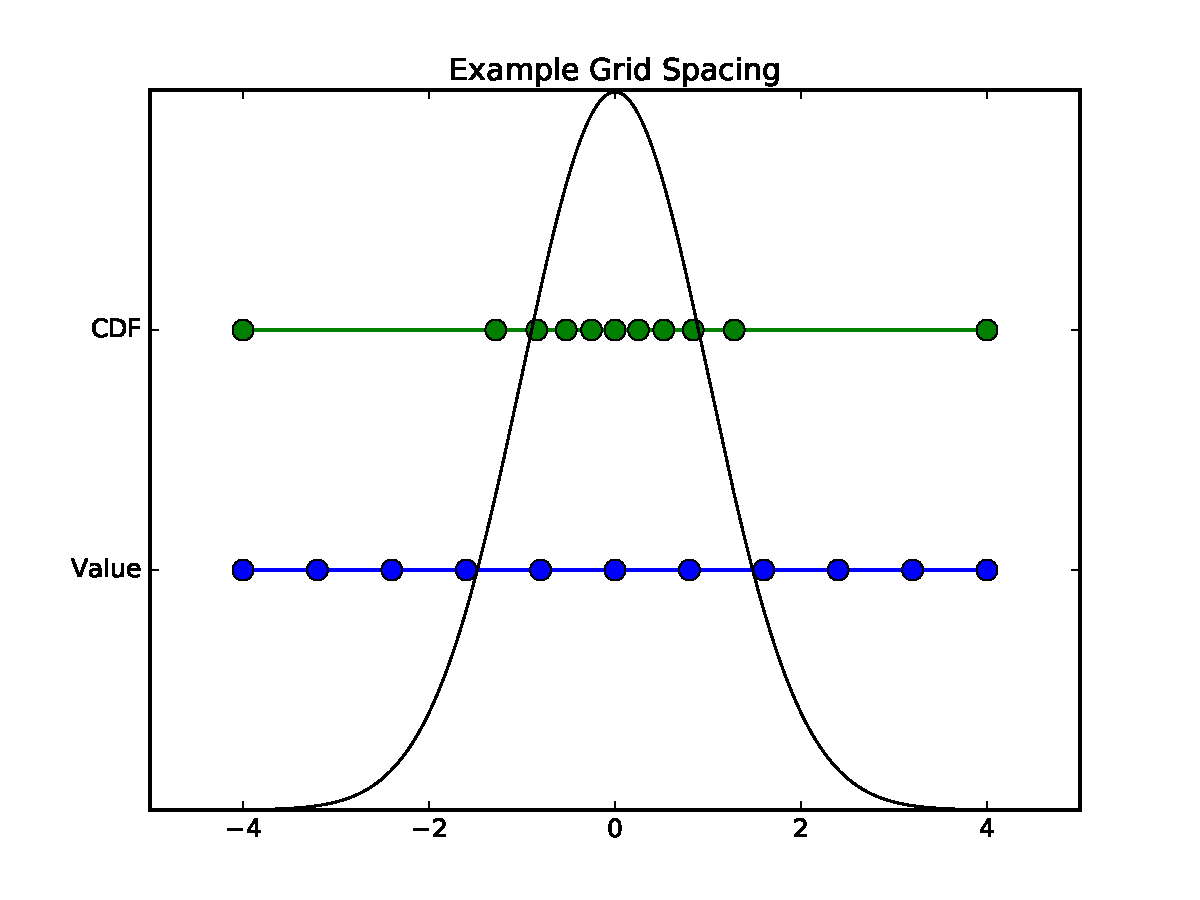
\includegraphics[width=0.7\linewidth]{grid_spacing}
  \caption{Grid Sampling}
  \label{fig:grid samp}
\end{figure}
In multidimensional input spaces, the tensor product of each grid is taken to result in the full grid.

Since the grid nodes are user-defined, approximating integrals are slightly more complicated than in the Monte
Carlo space.  The mean is approximated by
\begin{equation}
  \expv{u(Y)} = \int_\Omega \rho(Y) u(Y) dY \approx \sum_{m=1}^M w_m u(Y(\omega_m)),
\end{equation}
where $m$ iterates over each node in the grid, $Y(\omega_m)$ is the multidimensional input realization at grid node $m$, and
$w_m$ is a probability weight determined by the volume of probability represented by the grid node.  In grids
constructed by CDF, all $w_m$ are of the same value, while in grids spaced equally by value, $w_m$ can vary
significantly.  Similarly, the second moment is approximated by
\begin{equation}
  \expv{u(Y)^2} = \int_\Omega \rho(Y) u(Y)^2 dY \approx \sum_{m=1}^M w_m u(Y(\omega_m))^2.
\end{equation}

An advantage to grid sampling is its regular construction, which can give more clarity to how a response
behaves throughout the input space.  However, the grid construction suffers greatly from the curse of
dimensionality, which makes it inefficient for input spaces with large dimensionality.
Figure \ref{fig:grid sample}
shows Grid sampling of a two-dimensional input space, and Figure \ref{fig:grid prob} shows the
probability weight of the sampled points \cite{raven}.

\begin{figure}[H]
  \centering
  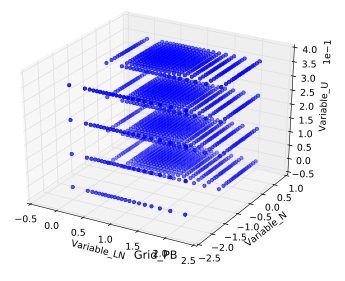
\includegraphics[width=0.5\linewidth]{grid_sample}
  \caption{Example Grid Samples \cite{raven}}
  \label{fig:grid sample}
\end{figure}
\begin{figure}[H]
  \centering
  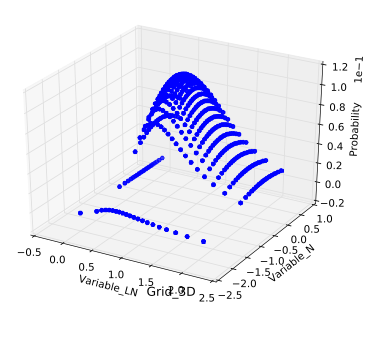
\includegraphics[width=0.5\linewidth]{grid_prob}
  \caption{Example Grid Probabilities \cite{raven}}
  \label{fig:grid prob}
\end{figure}


\subsection{LHS}
A cross between Monte Carlo and Grid sampling strategies, the Latin Hypercube Sampling (LHS) strategy 
is a sampling tool used to reduce
the total samples needed without significantly sacrificing integration quality \cite{lhs}.  In LHS, the input
space is also divided into a grid just as in the Grid sampling strategy.  However, unlike Grid sampling, only
one sample is taken per hyperplane; that is, for any of the input variables, there is only one sample taken
between each of the one-dimensional nodes.  Once a hypervolume is selected to take a sample, the exact
point is selected by random sampling in the probability space within the hypervolume.
Figure \ref{fig:lhs sample}
shows lhs sampling of a two-dimensional input space, and Figure \ref{fig:lhs prob} shows the
probability weight of the sampled points \cite{raven}.

\begin{figure}[H]
  \centering
  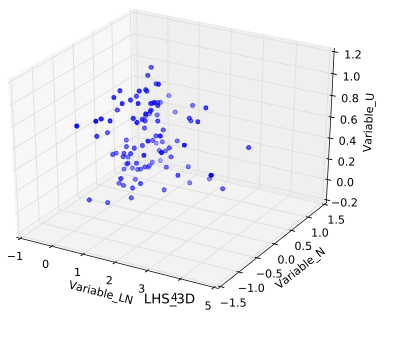
\includegraphics[width=0.5\linewidth]{lhs_sample}
  \caption{Example LHS Samples \cite{raven}}
  \label{fig:lhs sample}
\end{figure}
\begin{figure}[H]
  \centering
  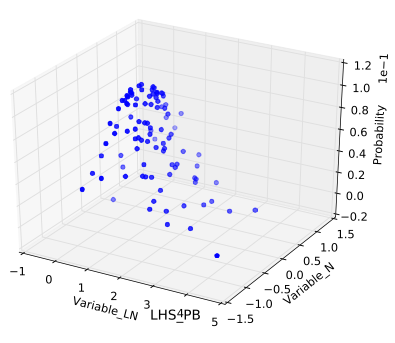
\includegraphics[width=0.5\linewidth]{lhs_prob}
  \caption{Example LHS Probabilities \cite{raven}}
  \label{fig:lhs prob}
\end{figure}

As in the Grid method, the weight of each sample is the probability volume of the hypervolume it represents.

